
\documentclass[../main/main.tex]{subfiles}
\usepackage{tikz}
\begin{document}

	
The fundamental design approach of this system is to layer several service on top of one another to add features. 
These layers are as follows; the database, the message server, the Tor hidden service, and the Ethereum authentication service. 
The goal of the message server is to receive and send http POST requests to other message servers on the network. 
Each device is used to act as its on message server and client. 
Using Tor hidden services to bypass the firewall on the local network allows for requests to be sent or received by other servers regardless of local network configurations \cite{TCP}.
To keep track of what address goes to what user an authentication service implemented on the Ethereum network is used to tie users to their TOR hidden service address. 
The database stores the information of the primary user, the user contacts, and the received messages.
Each is designed to work independently of the system below it, allow for more flexibility while implementing the application. 
In the following sections, the specific design of each layer will be reviewed.

\textbf{The Database} contains several tables: Primary user, Contacts, Conversations, and messages. 
Primary user is the user of the current instance of the application. 
Information regarding the address of their TOR hidden server and their username is stored in the primary user table. 
The Contacts table is used to store the contacts of the primary user, their associated shared keys, and the last updated address of the contact. 
The Conversations table stores the active conversations, associating the users with the conversations they are apart of.
Finally messages are stored in the message table which holds information on the conversation the message is apart of, the message itself, and a time stamp of when the message was received. 
The message server makes use of the database to store messages and look up conversations to validate received messages.

\textbf{The Message Server} is an http server which receives and sends HTTP post requests and uses SSL for further encryption of the data stream. 
Requests contain a JSON object with two fields: the conversation hash, and the hashed message. 
256SHA is used along with a key shared by each user to decode/hash the data.
The conversation hash is used to identify the conversation that the message belongs to.
Using this the unhashed name of the conversation the message server then inserts the message into the database storing the associated conversation id and a timestamp of when the message occurred.
To send messages the server again uses POST requests to transmit the data in the same fashion it received it, retrieving destination address from the database. 
One received the http server will return an OK as an acknowledgement
Each user acts as both client and server which forms the peer to peer structure of the network.
\begin{center}



\tikzset{every picture/.style={line width=0.75pt}} %set default line width to 0.75pt        

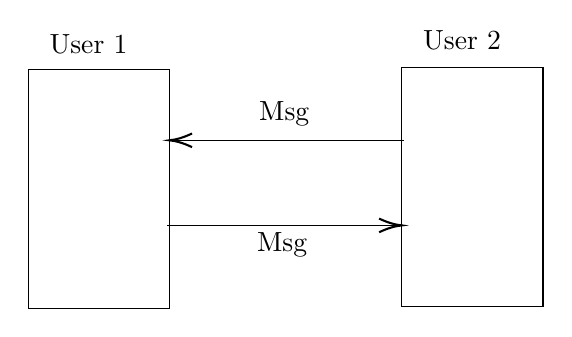
\begin{tikzpicture}[x=0.75pt,y=0.75pt,yscale=-1,xscale=1]
%uncomment if require: \path (0,300); %set diagram left start at 0, and has height of 300

%Shape: Rectangle [id:dp23235670811760722] 
\draw   (202,107) -- (270,107) -- (270,222) -- (202,222) -- cycle ;
%Shape: Rectangle [id:dp3647824809682021] 
\draw   (382,106) -- (450,106) -- (450,221) -- (382,221) -- cycle ;
%Straight Lines [id:da1599191724924538] 
\draw    (269,182) -- (380,182) ;
\draw [shift={(382,182)}, rotate = 180] [color={rgb, 255:red, 0; green, 0; blue, 0 }  ][line width=0.75]    (10.93,-3.29) .. controls (6.95,-1.4) and (3.31,-0.3) .. (0,0) .. controls (3.31,0.3) and (6.95,1.4) .. (10.93,3.29)   ;
%Straight Lines [id:da827215051818337] 
\draw    (383,141) -- (272,141) ;
\draw [shift={(270,141)}, rotate = 360] [color={rgb, 255:red, 0; green, 0; blue, 0 }  ][line width=0.75]    (10.93,-3.29) .. controls (6.95,-1.4) and (3.31,-0.3) .. (0,0) .. controls (3.31,0.3) and (6.95,1.4) .. (10.93,3.29)   ;

% Text Node
\draw (211,89) node [anchor=north west][inner sep=0.75pt]   [align=left] {User 1};
% Text Node
\draw (391,87) node [anchor=north west][inner sep=0.75pt]   [align=left] {User 2};
% Text Node
\draw (312,121) node [anchor=north west][inner sep=0.75pt]   [align=left] {Msg};
% Text Node
\draw (311,184) node [anchor=north west][inner sep=0.75pt]   [align=left] {Msg};


\end{tikzpicture}

\end{center}

\textbf{Tor} hidden services are used to facilitate connections to servers behind NATs without port forwarding in a method know as NAT hole punching \cite{TCP}. 
NAT stands for natural address translation, and is used to hide network IP ranges behind a single network address. 
They are needed because IPV4 only has a set number of IPs that can be assigned in a network. 
So by splitting larger networks up into their own isolated networks IPs can be reused. 
Many NATs and firewalls do not allow servers from outside the network to initiate connections inside the network. 
So for most messaging services like Imessage use centralized servers that devices can call out to retrieve data. 
Tor can be used to skip this intermediate step by acting as a rendezvous server \cite{TOR}. 
Devices behind NATs can reach out to these servers which in turn are able to forward incoming connections to the device.
This effectively is what as known as "TCP hole punching" and is what allows devices to act as their own message server. 
By making a TOR hidden service hosted on the device, incoming http post requests can be received by noctua message servers. 
The hidden service is separate from the message server and just transfers data between a listening port.

\begin{center}




\tikzset{every picture/.style={line width=0.75pt}} %set default line width to 0.75pt        

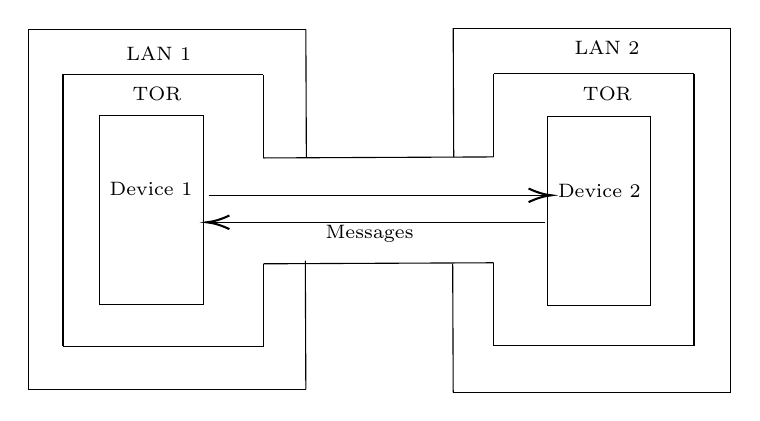
\begin{tikzpicture}[x=0.75pt,y=0.75pt,yscale=-1,xscale=1]
%uncomment if require: \path (0,300); %set diagram left start at 0, and has height of 300

%Shape: Rectangle [id:dp4095261685063052] 
\draw   (200.5,109.5) -- (250.5,109.5) -- (250.5,200.5) -- (200.5,200.5) -- cycle ;
%Shape: Rectangle [id:dp5309017293927076] 
\draw   (416,110) -- (466,110) -- (466,201) -- (416,201) -- cycle ;
%Straight Lines [id:da6455873511705832] 
\draw    (182.75,89.5) -- (182.75,220.5) ;
%Straight Lines [id:da3946202562243204] 
\draw    (182.75,90) -- (279.25,90) ;
%Straight Lines [id:da19484091602757014] 
\draw    (182.75,221) -- (279.25,221) ;
%Straight Lines [id:da33159699481361393] 
\draw    (390.25,220.5) -- (486.75,220.5) ;
%Straight Lines [id:da6977824325694792] 
\draw    (486.75,89.5) -- (486.75,220.5) ;
%Straight Lines [id:da8425870729550236] 
\draw    (390.25,89.5) -- (486.75,89.5) ;
%Straight Lines [id:da822280928441451] 
\draw    (279.25,90) -- (279.25,130) ;
%Straight Lines [id:da5681590281074294] 
\draw    (390.25,89.5) -- (390.25,129.5) ;
%Straight Lines [id:da5314723345146197] 
\draw    (279.25,181) -- (279.25,221) ;
%Straight Lines [id:da21964291915607714] 
\draw    (390.25,180.5) -- (390.25,220.5) ;
%Straight Lines [id:da31597706239703394] 
\draw    (279.25,130) -- (390.25,129.5) ;
%Straight Lines [id:da0233399602450175] 
\draw    (279.25,181) -- (390.25,180.5) ;
%Straight Lines [id:da7530764224188424] 
\draw    (299.75,68) -- (300,130) ;
%Straight Lines [id:da22899026775817632] 
\draw    (166,68) -- (299.75,68) ;
%Straight Lines [id:da6982663655952772] 
\draw    (166,68) -- (166,241.5) ;
%Straight Lines [id:da29329851570753385] 
\draw    (166,241.5) -- (299.75,241.5) ;
%Straight Lines [id:da11310324633583835] 
\draw    (299.5,179.5) -- (299.75,241.5) ;
%Straight Lines [id:da1764224174873601] 
\draw    (370.75,67.5) -- (371,129.5) ;
%Straight Lines [id:da1894746967753831] 
\draw    (370.75,67.5) -- (504.5,67.5) ;
%Straight Lines [id:da6621551434258164] 
\draw    (370.5,181) -- (370.75,243) ;
%Straight Lines [id:da7375386805321424] 
\draw    (370.75,243) -- (504.5,243) ;
%Straight Lines [id:da032210808783210476] 
\draw    (504.5,67.5) -- (504.5,243) ;
%Straight Lines [id:da4343897248863906] 
\draw    (253,148) -- (416,148) ;
\draw [shift={(418,148)}, rotate = 180] [color={rgb, 255:red, 0; green, 0; blue, 0 }  ][line width=0.75]    (10.93,-3.29) .. controls (6.95,-1.4) and (3.31,-0.3) .. (0,0) .. controls (3.31,0.3) and (6.95,1.4) .. (10.93,3.29)   ;
%Straight Lines [id:da27661390958898924] 
\draw    (415,161) -- (254,161) ;
\draw [shift={(252,161)}, rotate = 360] [color={rgb, 255:red, 0; green, 0; blue, 0 }  ][line width=0.75]    (10.93,-3.29) .. controls (6.95,-1.4) and (3.31,-0.3) .. (0,0) .. controls (3.31,0.3) and (6.95,1.4) .. (10.93,3.29)   ;

% Text Node
\draw (204,140.5) node [anchor=north west][inner sep=0.75pt]  [font=\scriptsize] [align=left] {Device 1};
% Text Node
\draw (420,141.5) node [anchor=north west][inner sep=0.75pt]  [font=\scriptsize] [align=left] {Device 2};
% Text Node
\draw (212,75.5) node [anchor=north west][inner sep=0.75pt]  [font=\scriptsize] [align=left] {LAN 1};
% Text Node
\draw (428,72.5) node [anchor=north west][inner sep=0.75pt]  [font=\scriptsize] [align=left] {LAN 2};
% Text Node
\draw (432,94.5) node [anchor=north west][inner sep=0.75pt]  [font=\scriptsize] [align=left] {TOR};
% Text Node
\draw (215,94.5) node [anchor=north west][inner sep=0.75pt]  [font=\scriptsize] [align=left] {TOR};
% Text Node
\draw (308,161) node [anchor=north west][inner sep=0.75pt]   [align=left] {{\scriptsize Messages}};


\end{tikzpicture}


\end{center}

\textbf{EAS}(Ethereum Authentication service) will be used as for identity management and name services. 
Using smart contracts to allow users to create a username and set an associated address securely. 
The EAS stores the last update address of the users Tor hidden service. With
each username being unique allowing for users to add contacts via usernames like they would with any other service. 
When a contact is added the application will attempt to initiate a transaction to find the user in the EAS. 
If found it will add its contact and address to the users hidden service. 
to keep address fresh, whenever a new hidden service is created, a new transaction will be initiated to update the users hidden service address. 
If a user sends a message to a contact and that contacts HTTP server does not respond another transaction will attempt to find the new address of the contact.
Due to the nature of the Ethereum network transactions are automatically authenticated by the network using the users wallet address \cite{ETH} meaning only the user can update their own addresses.


\end{document}